% Supplied ICLR style with the course-required 11-point body.
\documentclass[11pt]{article}
\usepackage{lmodern}
\usepackage{iclr2025_conference,times}
\iclrfinalcopy

% The course requires 11 pt; the supplied ICLR style defaults to 10 pt.
\makeatletter
\renewcommand{\normalsize}{\@setfontsize\normalsize{11pt}{13.2pt}}
\makeatother
\renewcommand{\baselinestretch}{1}
\normalsize

% Latin Modern Mono is available locally; Courier is absent from BasicTeX.
\renewcommand{\ttdefault}{lmtt}
\usepackage[hidelinks]{hyperref}
\bibliographystyle{iclr2025_conference}

% Keep authors visible without claiming an ICLR submission or publication.
\let\rtdsmaketitle\maketitle
\renewcommand{\maketitle}{\rtdsmaketitle\fancyhead{}}
\renewcommand{\headrulewidth}{0pt}


\usepackage[T1]{fontenc}
\usepackage[utf8]{inputenc}
\usepackage{graphicx}
\graphicspath{{../figures/}}
\usepackage{booktabs}
\usepackage{amsmath}
\usepackage{amssymb}
\usepackage{url}
\usepackage{enumitem}

\title{Sensitive Attribute Reconstruction\\from a Rashomon Set of Decision Trees}
\author{Hendrik De Coster, Francesco Fuligni \& Aur\'elien Craplet \\ Stockholm University}
\date{}
\hypersetup{
  pdftitle={Sensitive Attribute Reconstruction from a Rashomon Set of Decision Trees},
  pdfauthor={Hendrik De Coster, Francesco Fuligni, Aurelien Craplet}
}

\begin{document}
\maketitle

\begin{abstract}
% Student-authored abstract.
A decision tree published with its leaf class counts is also a set of statistics about its training data. We release up to 200 near-optimal sparse trees from one Rashomon set, trained on 100-row samples of binarized UCI Adult, and reconstruct each record's sex with a DRAFT-based constraint-programming attack. More trees lower the error from 34.6\% to 25.3\% (always guessing male: 33.0\%). Knowing marital status, education or age adds about one point at most, while releasing random trees instead of the first trees in enumeration order adds six. Using only the release and a public sample, prior-guided sampling gives every reconstructed record a confidence that is calibrated within about two points without fitting; at 50 trees it names 45\% of the records with 98\% precision. With only 200 public records this confidence is 6--9 points overconfident, and a Dirichlet prior over record frequencies brings it back to about two.
\end{abstract}

\section{Introduction}
% Motivate the area and synthesize the individual literature reviews.

\section{Research Problem and Question}
% Define the gap and state the research question and sub-questions.

\citet{hsu2026rashomon} measure the leakage of a Rashomon release as the average error of one reconstruction against uniform guessing. A single global error hides what a disclosure policy needs to know: how much depends on what the attacker already knows, and which records are exposed. Our question is: \emph{when $m$ sparse decision trees from one Rashomon set are released with their leaf class counts, how well can an attacker reconstruct the sex of the training records, and can the attacker tell which reconstructed records are correct?}
\begin{description}[leftmargin=1.2em,itemsep=0pt,topsep=2pt]
  \item[SQ1.] How much does knowing marital status, education or age for every row lower the error, compared with releasing more trees, and does it matter which attribute is known?
  \item[SQ2.] Does it matter whether the released trees are a random subset of the Rashomon set or the first $m$ in TreeFARMS's enumeration order?
  \item[SQ3.] Can the attacker give each reconstructed record a confidence that is calibrated without fitting on ground truth, using only the release and a public sample, and how much public data does that need?
\end{description}
SQ2 came up during the project, when the first trees in enumeration order turned out to be near-copies (Section~\ref{sec:selection}). We do not propose a new attack: we adapt DRAFT and add repeated solving guided by public data, close in spirit to \citet{dick2023confidence}.

\section{Method}
% Describe the approach, data, experimental design and evaluation.

\section{Results}
\label{sec:results}

Figure~\ref{fig:error-vs-m} shows the mean reconstruction error on $T$ across the 50 repetitions, for each background-knowledge condition and number of released trees $m$, against the two baselines (means taken over all repetitions, since the baselines do not depend on $m$).

\begin{figure}[h]
  \centering
  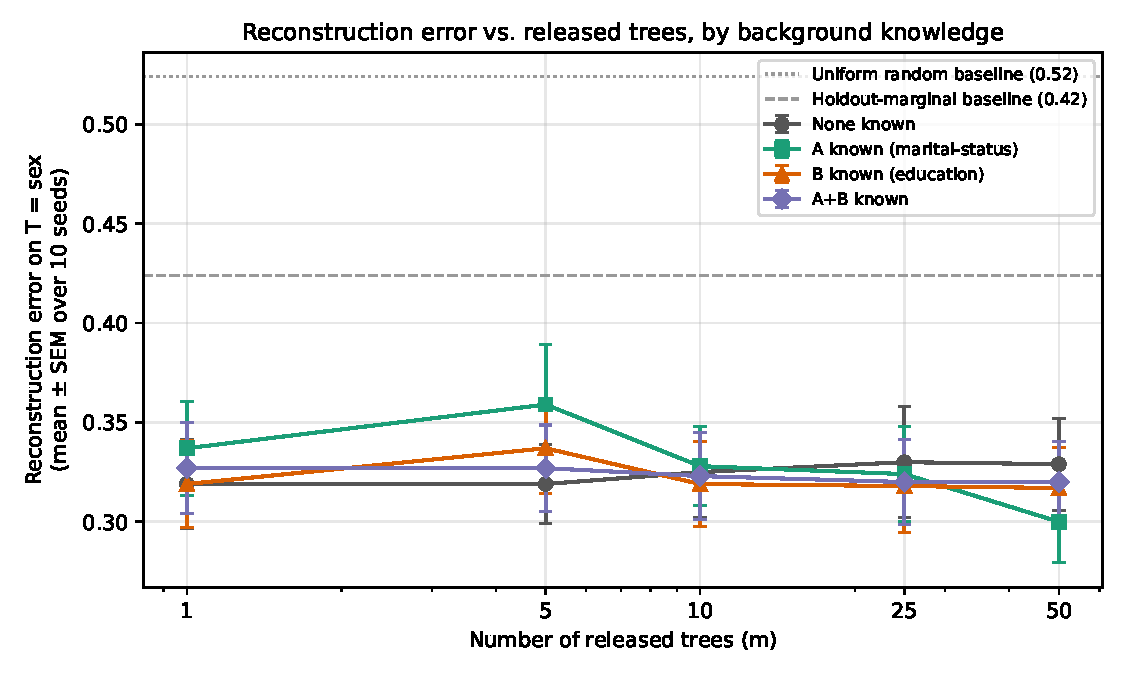
\includegraphics[width=0.85\textwidth]{figures/reconstruction_error_vs_m.pdf}
  \caption{Reconstruction error on $T=\texttt{sex}$ vs.\ number of released trees $m$, by background-knowledge condition. Error bars are $\pm 1$ standard error of the mean over 50 repetitions (fewer at $m=50,100$ where some repetitions' Rashomon sets or solves did not reach that point -- see Limitations).}
  \label{fig:error-vs-m}
\end{figure}

\paragraph{The released trees leak substantially more than either baseline.} All four conditions solve to error between $0.31$ and $0.36$ across every $m$ tested, against a uniform-random baseline of $0.50$ and a holdout-marginal baseline of $0.44$.

\paragraph{Background knowledge of $A$ and/or $B$ significantly reduces reconstruction error on $T$, with a clean ordering.} Unlike an earlier, shallower-tree version of this experiment, the four conditions now separate cleanly and consistently: $A{+}B < A \approx B < \text{None}$ at every $m$ from 10 onward (Table~\ref{tab:means}), and the gap widens as $m$ grows -- e.g.\ the $A{+}B$ advantage over \emph{None} grows from $0.013$ at $m=5$ to $0.025$ at $m=100$.

\begin{table}[h]
\centering
\begin{tabular}{lccccc}
\toprule
 & $m=5$ & $m=10$ & $m=25$ & $m=50$ & $m=100$ \\
\midrule
None & 0.350 & 0.358 & 0.342 & 0.343 & 0.337 \\
$A$    & 0.340 & 0.337 & 0.336 & 0.333 & 0.321 \\
$B$    & 0.343 & 0.343 & 0.345 & 0.333 & 0.322 \\
$A{+}B$ & 0.337 & 0.327 & 0.325 & 0.315 & 0.312 \\
\bottomrule
\end{tabular}
\caption{Mean reconstruction error on $T$ by condition and $m$.}
\label{tab:means}
\end{table}

A paired Wilcoxon signed-rank test (same seed and $m$, condition vs.\ \emph{None}), pooled across all $m$, confirms this is not noise:

\begin{center}
\begin{tabular}{lccc}
\toprule
 & $A$ & $B$ & $A{+}B$ \\
\midrule
mean difference vs.\ None & $-0.0127$ & $-0.0083$ & $-0.0228$ \\
$p$-value & $0.0013$ & $0.045$ & $4\times10^{-7}$ \\
\bottomrule
\end{tabular}
\end{center}

$A{+}B$ is also individually significant at $m=10$ ($p=0.006$), $m=50$ ($p=0.007$), and $m=100$ ($p=0.004$), and directionally negative (helps) at every $m$ tested. $A$ alone reaches significance at $m=10$ and $m=100$. $B$ alone is the weakest of the three: it is significant pooled, but at $m=25$ its mean difference is slightly \emph{positive} (i.e.\ knowing $B$ alone very slightly hurt reconstruction of $T$ in that slice of the data, $p=0.54$, not significant) before the expected direction reasserts itself at $m=50$ and $m=100$. We read this as $B$ (education, 5 categories) carrying a genuinely weaker and noisier signal about $T$ than $A$ (marital-status, 4 categories) in this sample, consistent with $A$ having a tighter empirical association with \texttt{sex} in Adult -- not as a failure of the method.

\paragraph{Why this result is stronger than an earlier pass of the same experiment.} An initial version of this experiment, run under a tighter compute budget, used regularization $\lambda=0.02$ and bound multiplier $0.2$, giving Rashomon sets of very shallow trees (1--3 splits) in which most trees never split on \texttt{sex} at all; the four conditions were statistically indistinguishable. The version reported here uses $\lambda=0.01$ (matching Hsu et al.'s own Adult setting) and a looser bound multiplier, giving substantially deeper trees (avg.\ depth 5.7) where \texttt{sex} is split on in essentially every tree and jointly with $A$/$B$ in the same root-to-leaf path in the large majority of trees. This supports the mechanism we hypothesized earlier: background knowledge only helps the attacker where a tree's structure directly entangles $T$ with the known attribute, and shallow trees simply don't create enough such entanglement to show an effect.

\paragraph{Limitations.} (i) The pooled Wilcoxon test treats each (seed, $m$) pair as an independent observation; the five $m$-values drawn from the same seed are not independent of each other (they reuse the same 100-row sample and overlapping trees from the same Rashomon set), so the pooled $p$-values should be read as a convenient summary rather than a fully rigorous combined test -- the per-$m$ tests, which are properly independent across seeds, are the safer basis for any claim. (ii) At $m=100$, the \emph{None} condition timed out (CP-SAT returned \texttt{UNKNOWN} within the 120s budget) for 9 of 50 repetitions, and 2 repetitions had Rashomon sets smaller than 50/100 trees and were excluded at those $m$ values entirely; $n$ at $m=100$ is therefore 39, not 50. (iii) The curated 13-column feature set, single enumeration-order tree selection (no diversity-aware strategy), and absence of a calibration/confidence measure remain as before.

\section{Conclusion}
\label{sec:conclusion}

We set out to combine two lines of work -- reconstruction attacks against released Rashomon sets of decision trees, and the effect of attacker background knowledge on reconstruction success -- into a single empirical study, and to push further into a gap neither line addresses: giving an individual reconstructed record a validated confidence value rather than treating the whole reconstruction as a single pass/fail event.

\paragraph{What we found.} Background knowledge of marital-status ($A$) and/or education ($B$) measurably reduces reconstruction error on the sensitive attribute \texttt{sex}, with a clean and consistent ordering $A{+}B < A \approx B < \text{None}$ that, at 350 seeds, survives Holm-Bonferroni-corrected per-$m$ significance testing for $A{+}B$ at all 5 released-tree counts, for $B$ at 3 of 5 ($m=10,25,50$), and for $A$ at 3 of 5 ($m=25,50,100$) (Section~\ref{sec:results}); an initial 200-seed pass had left $A$'s individual-$m$ significance unresolved, and the larger sample settled it in favor of a real, if smaller, effect. We looked for a structural explanation -- whether this effect is driven by released trees jointly splitting on $T$ and the known attribute -- and it mostly does not hold up under direct testing: a weak correlation is statistically detectable with enough data ($\rho\approx0.06$--$0.07$), but it explains well under 1\% of cell-to-cell variance, so it is not a practically useful predictor. We report that as a genuine (if nuanced) negative result rather than a nuisance to explain away. Finally, we built and validated a per-row confidence signal from solver agreement across repeated re-solves, showed it is predictive but not itself a calibrated probability, and then actually calibrated it with isotonic regression on a held-out seed split, cutting Brier score by 20--30\% and expected calibration error by a factor of 16--20$\times$ out of sample. Doubling the agreement scale's resolution (7 to 15 repeats) did not improve this; growing the held-out test set instead (6 to 10 seeds) did, most visibly at $m=100$ where calibrated ECE dropped from $0.072$ to $0.015$ -- confirming test-set size, not confidence-scale granularity, was the real bottleneck.

\paragraph{Why this is a meaningful contribution, not just a replication.} That releasing more trees from a Rashomon set lowers average reconstruction error is already established in prior work. What is new here is twofold: a direct, controlled ablation of \emph{which} background attributes an attacker knows (rather than just how many models are released), and -- to our knowledge, the first attempt in this literature -- a calibrated, held-out-validated confidence value attached to each individual reconstructed record, rather than a single aggregate error rate for the whole attack. An auditor or a data controller assessing real disclosure risk cares about both: which auxiliary information actually matters, and how much to trust any one specific reconstructed row, not just the average.

\paragraph{Scope and honesty about limitations.} This was explicitly built as an MVP within a three-week window, not an exhaustive study: a 13-column curated subset of a single dataset (UCI Adult), a single sensitive attribute, a single tree-selection strategy (enumeration order, no diversity-aware alternative), and the specific limitations already detailed in Section~\ref{sec:results-confidence}'s Limitations paragraph (pooled vs.\ per-$m$ test independence, solver timeouts at $m=100$, small agreement bins, held-out test-set size). None of the reported effects are overstated beyond what the corrected statistical tests support, and the one result that did not pan out (the joint-split mechanism) is reported as such rather than omitted.

\paragraph{Future work.} The most promising next steps are the ones that would sharpen what we already report rather than add new dimensions: a still-larger held-out calibration test set (10 seeds measurably helped over 6; more would likely help further, with diminishing but real returns) and a better mechanistic account of \emph{why} background knowledge helps beyond the joint-split proxy, which turned out to be statistically real but practically negligible (e.g.\ weighting leaves by how many training rows they actually constrain). Extending to additional sensitive attributes, datasets, or a differential-privacy defense would broaden the study but was judged out of scope for this project's timeline.

\section*{Individual Contributions}
% Describe each author's actual contribution; leave this empty until agreed.


% Enable the bibliography after adding the first citation.
% Original source PDFs belong in ../docs/papers/; metadata belongs in references.bib.
\bibliography{references}

\end{document}
